\subsubsection{Example: Math achievement and SES}

To illustrate, we use the classic data set from %Bryk \& Raudenbush (2002)
\citet{BrykRaudenbush:1992,RaudenbushBryk:2002}
dealing with math achievement scores from a subsample of 7,185 students from 160 schools
in a 1982 High School \& Beyond survey of U.S. public and Catholic high
schools conducted by the National Center for Education Statistics (NCES).
The data set contains 90 public schools and 70 Catholic schools, with
sample sizes ranging from 14 to 67.

The response is a standardized measure of math achievement, while
student-level predictor variables include Sex and student SES, and
school-level predictors include Sector (public or Catholic) and mean SES for the
school (among other variables).
Following \citet{RaudenbushBryk:2002}, student SES is considered the main predictor, and is 
typically analyzed in centered form,
CSES = SES - meanSES for ease of interpretation (making the within-school intercept
equal to meanSES for that school).



\begin{figure}[htb]
 \begin{minipage}[b]{.49\linewidth}
  \centering
  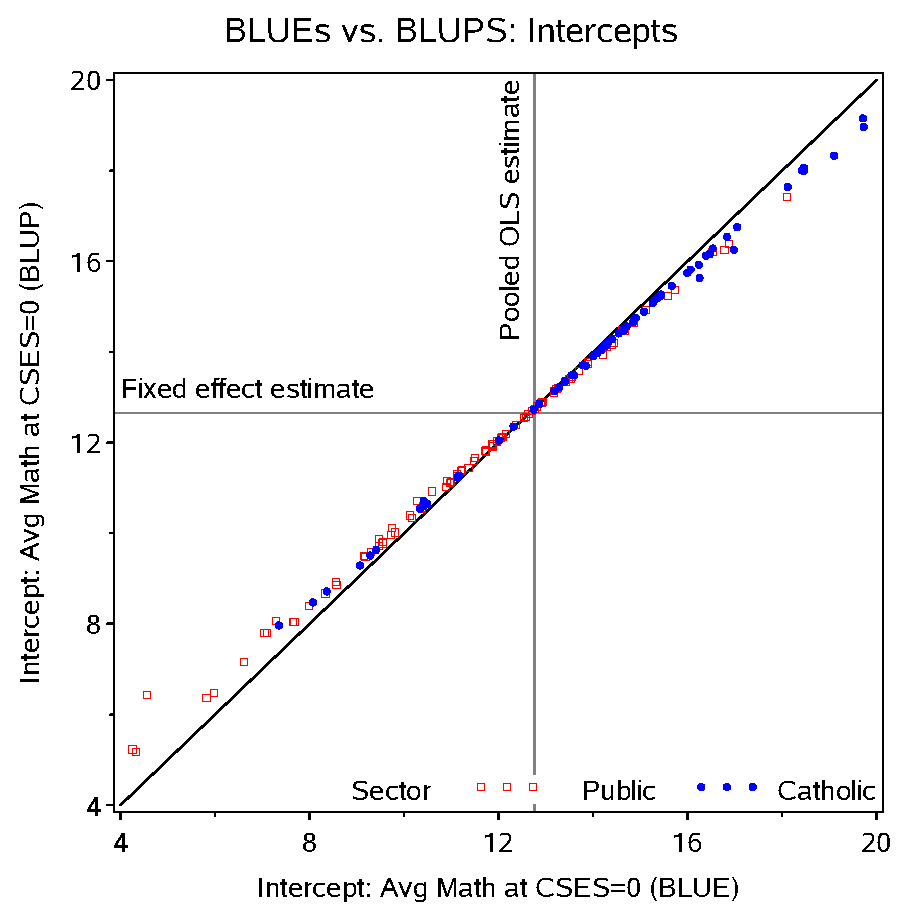
\includegraphics[width=1\linewidth,clip]{fig/hsbmix41}
%  \caption{}%
%  \label{fig:}
 \end{minipage}%
 \hfill
 \begin{minipage}[b]{.49\linewidth}
  \centering
  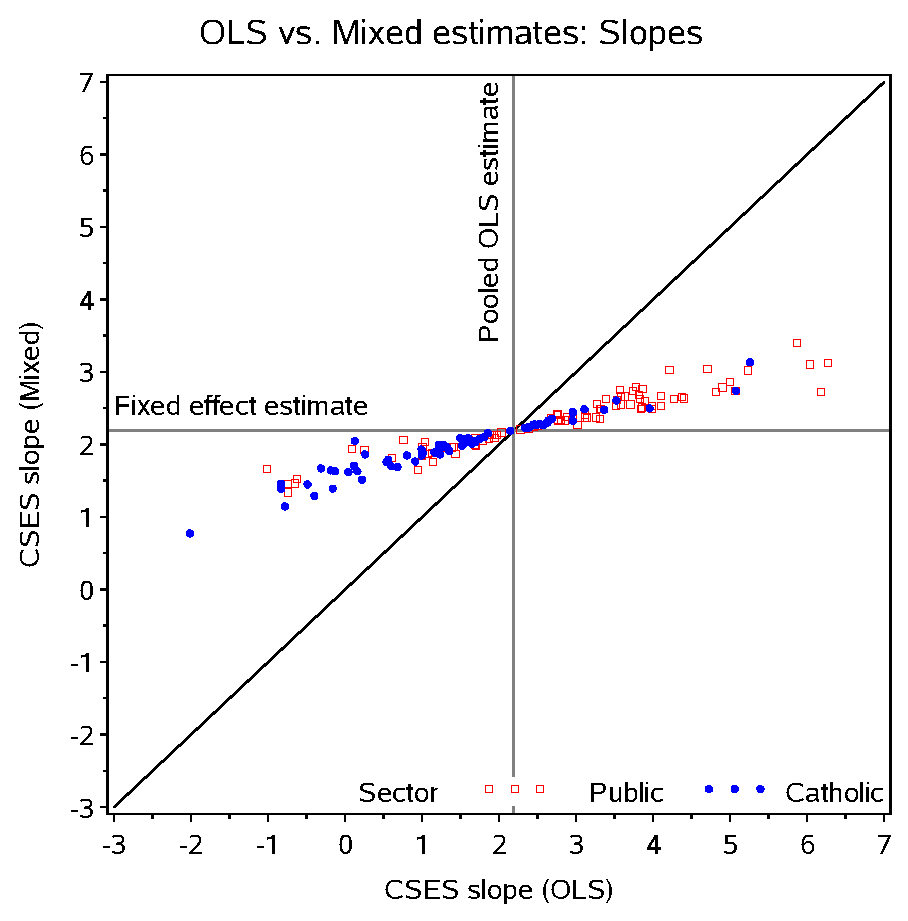
\includegraphics[width=1\linewidth,clip]{fig/hsbmix42}
 \end{minipage}
  \caption{Comparing BLUEs and BLUPs. Each panel plots the OLS estimates from separate regressions for each school (BLUEs)
  versus the mixed model estimates from the random intercepts and slopes model (BLUPs).
  Left: intercepts; Right: slopes for CSES.  The shrinkage of the BLUPs toward the OLS estimate is much greater for slopes than
  intercepts. }
  \label{fig:hsbmix4}
\end{figure}


\begin{figure}[htb!]
  \centering
  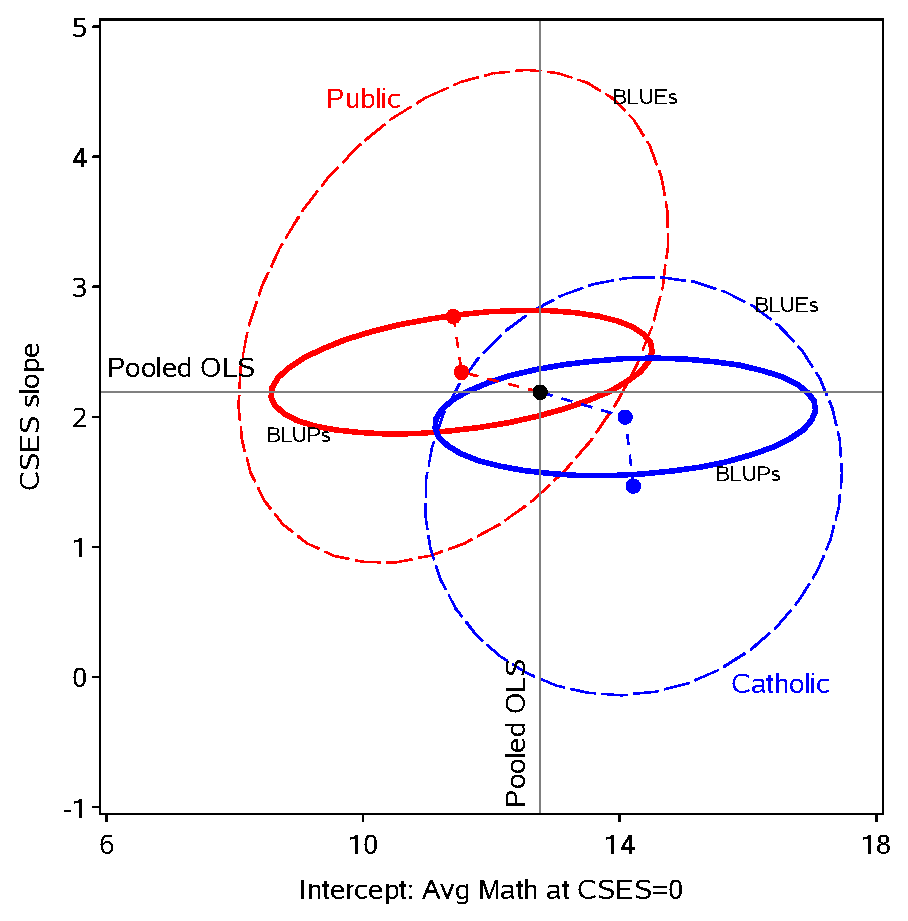
\includegraphics[width=.6\textwidth,clip]{fig/hsbmix43}
  \caption{Comparing BLUEs and BLUPs. The plot shows ellipses of 50\% coverage for the estimates of intercepts and slopes
  from OLS regressions (BLUEs) and the mixed model (BLUPs), separately for each sector.
  The centers of the ellipses illustrate how the BLUPS can be considered a weighted average of the BLUEs and the
  pooled OLS estimate, ignoring sector. The relative sizes of the ellipses reflect the smaller variance for the
  BLUPs compared to the BLUEs, particularly for slope estimates. }%
  \label{fig:hsbmix43}
\end{figure}
